\documentclass[10pt,showpacs,preprintnumbers,footinbib,amsmath,amssymb,aps,prl,twocolumn,groupedaddress,superscriptaddress,showkeys]{revtex4-1}
\usepackage{graphicx}
\usepackage{dcolumn}
\usepackage{bm}
\usepackage[colorlinks=true,urlcolor=blue,citecolor=blue]{hyperref}
\usepackage{color}
\usepackage{listings}

\lstset{ %
  basicstyle=\footnotesize,        % the size of the fonts that are used for the code
  breakatwhitespace=false,         % sets if automatic breaks should only happen at whitespace
  breaklines=true,                 % sets automatic line breaking
  captionpos=t,                    % sets the caption-position to bottom
  deletekeywords={...},            % if you want to delete keywords from the given language
  escapeinside={\%*}{*)},          % if you want to add LaTeX within your code
  extendedchars=true,              % lets you use non-ASCII characters; for 8-bits encodings only, does not work with UTF-8
  frame=single,                    % adds a frame around the code
  keepspaces=true,                 % keeps spaces in text, useful for keeping indentation of code (possibly needs columns=flexible)
 % language=Python,                 % the language of the code
  morekeywords={*,...},           % if you want to add more keywords to the set
  numbers=left,                    % where to put the line-numbers; possible values are (none, left, right)
  numbersep=5pt,                   % how far the line-numbers are from the code
  showspaces=false,                % show spaces everywhere adding particular underscores; it overrides 'showstringspaces'
  showstringspaces=false,          % underline spaces within strings only
  showtabs=false,                  % show tabs within strings adding particular underscores
  stepnumber=1,                    % the step between two line-numbers. If it's 1, each line will be numbered
  tabsize=2,                       % sets default tabsize to 2 spaces
}


\begin{document}
\title{FYS3150 Computational Physics - Project 2}
\author{Nicholas Karlsen}

\begin{abstract}
  This is an abstract
\end{abstract}

\maketitle

\section{Introduction}
\section{Theory, Algorithms and Methods}
  \subsection{Preservation of scalar product \& orthogonality in unitary transformations\label{subsec:preservation}}
    Consider an orthonormal set of basis vectors $\mathbf v_i$ such that $\mathbf v_j^T \mathbf v_i = \delta_{ij}$. Let unitary matrix $U$ where $U^T U= I_N$, where $I_N$ denotes the $N\times N$ identity matrix, operate on $\mathbf v_i$ to get $\mathbf w_i$
    \begin{equation}
      \mathbf w_i = U \mathbf v_i
    \end{equation}
    Then
    \begin{equation}
      \mathbf w_j^T\mathbf w_i = (U\mathbf v_j)^TU\mathbf v_i = \mathbf v_j^T U^T U \mathbf v_i
      = \mathbf v_j^T \mathbf v_i = \delta_{ij}
    \end{equation}
    In the unitary transformation of $\mathbf v_i$ both the scalar product and orthogonality has been preserved.

\subsection{Givens rotation}
  A Givens rotation is a unitary transformation which performs a rotation in the plane spanned by two coordinate axes, represented by the matrix in Eqn. \ref{eqn:givens}.
  \begin{equation}
    \label{eqn:givens}
    G(i, j, \theta) = 
    \begin{bmatrix}
      1 & \dots & 0 & \dots & 0 & \dots & 0 \\
      \vdots & \ddots & \vdots & & \vdots & & \vdots \\
      0 &\dots & \cos\theta & \dots  & - \sin \theta & \dots & 0 \\
      \vdots && \vdots & \ddots & \vdots && \vdots \\
      0 & \dots & \sin \theta & \dots & \cos \theta & \dots & 0 \\
      \vdots && \vdots && \vdots & \ddots & \vdots \\
      0 & \dots & 0 & \dots & 0 & \dots & 1
    \end{bmatrix}
  \end{equation}
  where nonzero entries $g_{kk}=1$ for $k\neq i,j$, $g_{kk}=cos\theta$ for $k=i,j$ and $g_{ji} = -g_{ij} = -\sin \theta$ \cite{givens}

  As the Givens transformation it unitary, it also follows that it preserves both the scalar product and orthogonality, as shown in the section prior.

\subsection{Jacobi Eigenvalue Algorithm \label{subsec:jacobi_algo}}
    The jacobi eigenvalue algorithm finds the eigenpairs of real, symmetric matrices by diagonalization with Givens rotation matrix.

\section{Results and Discussions}
  \begin{figure}[h!]
    \center
    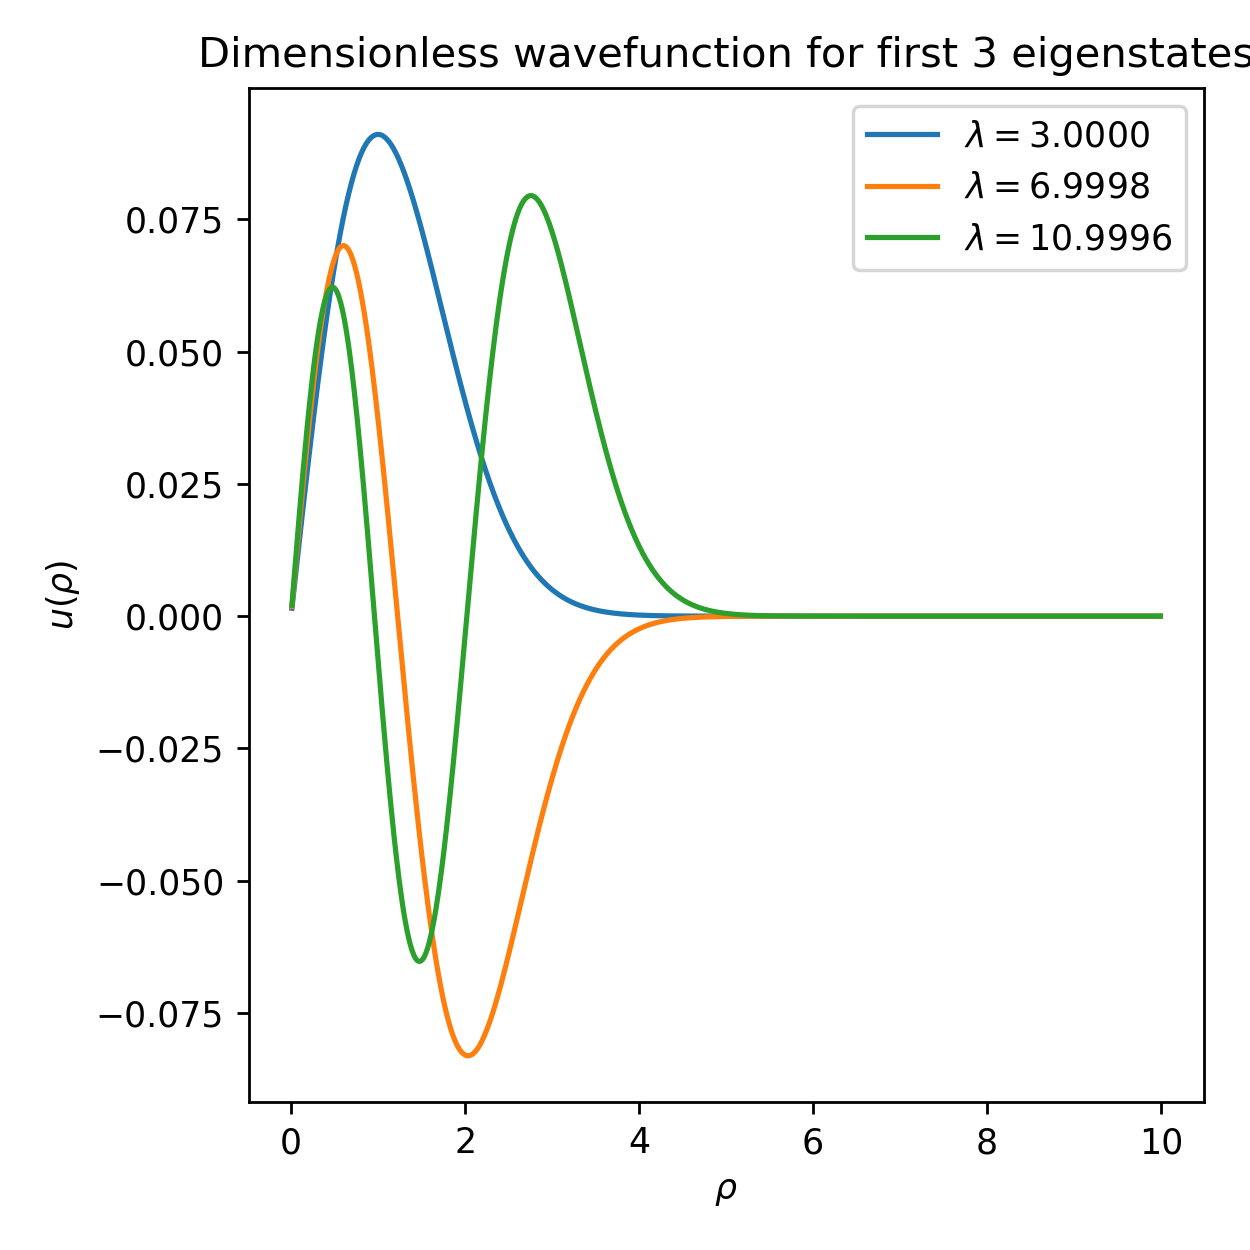
\includegraphics[width=8cm]{figs/question2d.png}
    \caption{First 3 eigenpairs in the solution of the harmonic oscillator potential for $N=1000$}
  \end{figure}

  \begin{figure}[h!]
    \center
    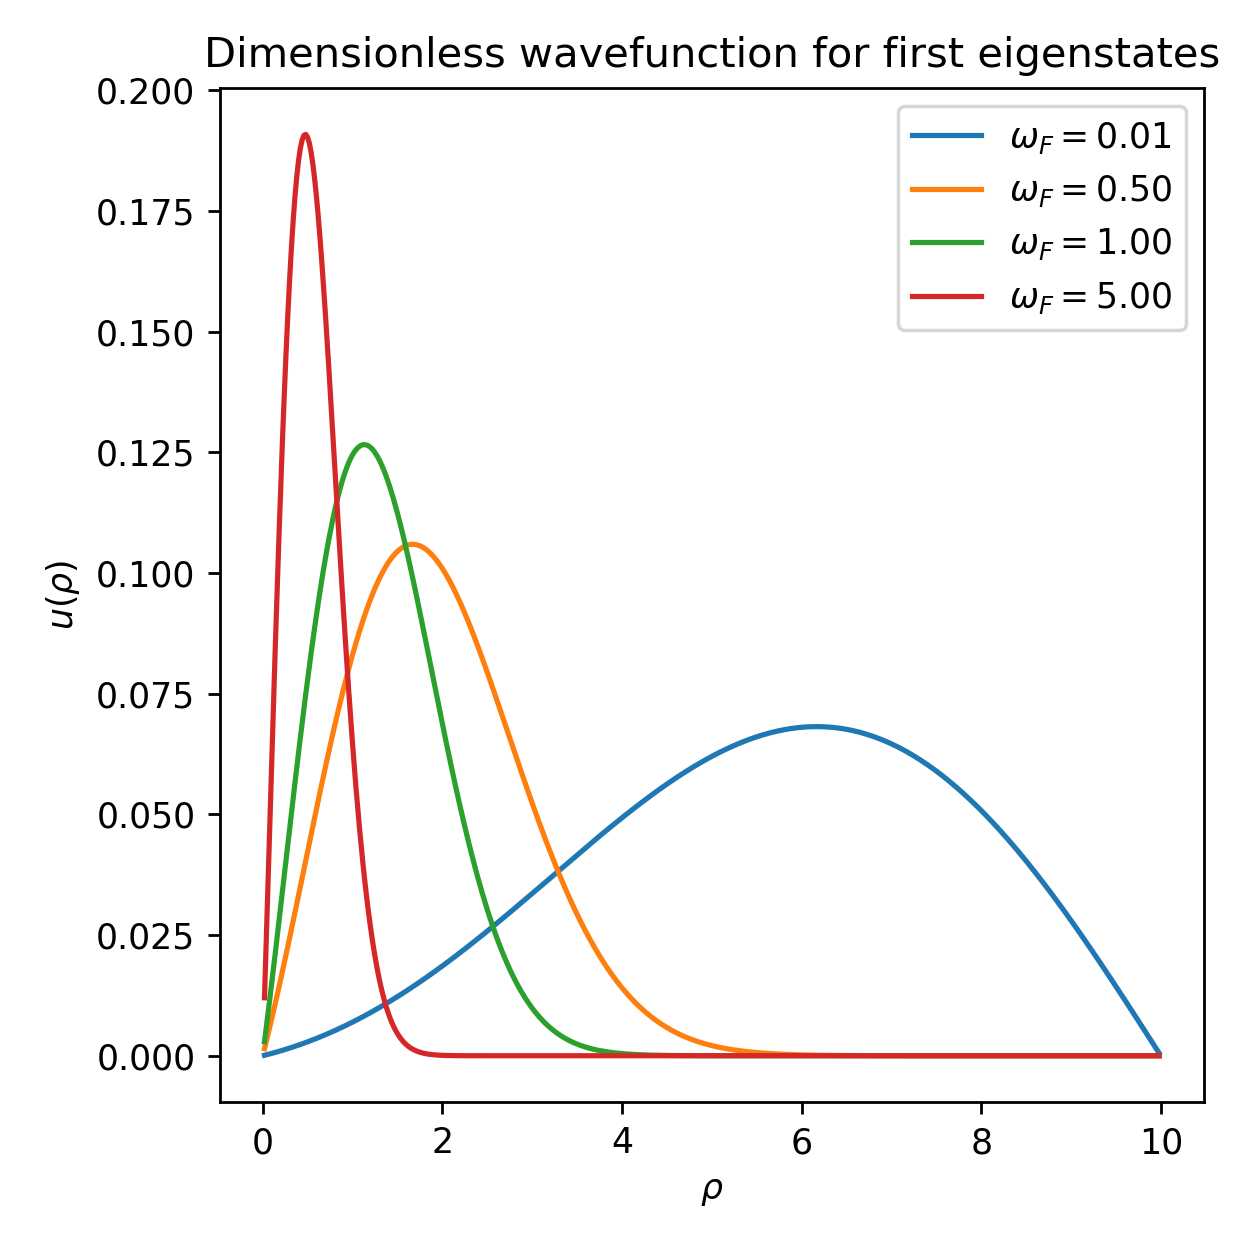
\includegraphics[width=8cm]{figs/question2e.png}
    \caption{...}
  \end{figure}


\section{Conclusions}

\begin{thebibliography}{99}
\bibitem{lecture_notes} M.~Hjorth-Jensen, Computational Physics - Lecture Notes 2015, (2015).
\bibitem{givens} Wikipedia contributors, Givens rotation --- {Wikipedia}{,} The Free Encyclopedia, [Online; accessed 1-October-2018]
\end{thebibliography}

\newpage
\appendix
\section{Jacobi Eigenvalue Algorithm}
\begin{lstlisting}[mathescape=true, language=python]
$\tau = \frac{a_{ll} - a_{kk}}{2a_{kl}}$

if $\tau \geq 0$:
    $t = \frac{1}{\tau + \sqrt{1 + \tau^2}}$
else:
    $t = \frac{-1}{-\tau + \sqrt{1 + \tau^2}}$

$c = \frac{1}{\sqrt{1 + t^2}}$
$s = tc$

$a_{kk}' = a_{kk}$
$a_{ll}' = a_{ll}$

$a_{kk} = c^2 * a_{kk}' - 2cs * a_{kl} + s^2 * a_{ll}'$
$a_{ll} = s^2 * a_{kk}' + 2cs * a_{kl} + c^2 * a_{ll}'$
$a_{kl} = 0.0 $
$a_{lk} = 0.0 $

for $i = 1, 2, \dots N$:
    if $i \neq k$ and $i \neq l$:
        $a_{ik} = a_{ik} $
        $a_{il} = a_{il} $
        $a_{ik} = c * a_{ik} - s * a_{il} $
        $a_{ki} = a_{ik} $
        $a_{il} = c * a_{il} + s * a_{ik} $
        $a_{li} = a_{il} $
\end{lstlisting}

\end{document}  